\subsubsection{Kebutuhan Fungsional}
Berikut merupakan kebutuhan fungsional dari sistem yang akan dibuat, agar lebih jelas kebutuhan fungsional dibuat ke dalam bentuk tabel di bawah ini. Semua kebutuhan fungsional akan memiliki ID yang diawali dengan huruf F lalu diikuti dengan dua angka.

\begin{table}
  \caption{Kebutuhan Fungsional}
  \label{tab:kebutuhan-fungsional}
  \centering
  \begin{tabular}{|c|p{4.5cm}|p{8cm}|}
    \hline
    ID  & Kebutuhan                                                                      & Penjelasan                                                                                                 \\
    \hline
    F01 & Sistem dapat meregistrasi perusahaan                                           & Admin dapat melakukan registrasi perusahaan baru ke dalam database sistem.                                 \\
    \hline
    F02 & Sistem dapat melihat seluruh perusahaan yang terdaftar                         & Admin dapat melihat seluruh perushaan yang ada pada database sistem.                                       \\
    \hline
    F03 & Sistem dapat melihat detail perusahaan                                         & Pengguna dapat melihat detail dari perushaan yang ada pada database sistem.                                \\
    \hline
    F04 & Sistem dapat melihat seluruh pengguna pada suatu perusahaan                    & Pengguna dapat melihat pengguna lain pada satu perusahaan yang sama                                        \\
    \hline
    F05 & Sistem dapat meregistrasi pengguna                                             & Admin dapat melakukan registrasi pengguna baru ke sebuah perusahaan pada sistem.                           \\
    \hline
    F06 & Sistem dapat menghapus pengguna                                                & Admin dapat menghapus pengguna dari suatu perusahaan                                                       \\
    \hline
    F07 & Sistem dapat melakukan authentikasi pengguna                                   & Pengguna dapat masuk ke dalam sistem dengan memasukan kredensial yang diberikan.                           \\
    \hline
    F08 & Sistem dapat menghapus authentikasi pengguna                                   & Pengguna dapat \textit{logout} dari sistem.                                                                \\
    \hline
    F09 & Sistem dapat meregistrasi perangkat \textit{IoT}                               & Pengguna dapat melakukan registrasi perangkat ke database sistem                                           \\
    \hline
    F10 & Sistem dapat melihat perangkat yang terdaftar                                  & Pengguna dapat melihat seluruh perangkat yang telah didaftarkan pada perushaannya                          \\
    \hline
    F11 & Sistem dapat menghapus perangkat yang terdaftar                                & Pengguna dapat menghapus perangkat yang telah didaftarkan di database                                      \\
    \hline
    F12 & Sistem dapat membuat \textit{groups}                                           & Pengguna dapat membuat \textit{groups} untuk mengelompokan beberapa perangkat                              \\
    \hline
    F13 & Sistem dapat melihat seluruh \textit{groups} yang telah didaftarkan            & Pengguna dapat melihat seluruh \textit{groups} yang telah terdaftar pada perusahannya                      \\
    \hline
    F14 & Sistem dapat menghapus \textit{groups} yang telah didaftarkan                  & Pengguna dapat menghapus \textit{groups} yang telah terdaftar pada perusahannya                            \\
    \hline
    F15 & Sistem dapat melihat seluruh perangkat yang terasosiasi dengan \textit{groups} & Pengguna dapat melihat hubungan antara perangkat dan \textit{groups} pada sistem dan begitupula sebaliknya \\
    \hline
    F16 & Sistem dapat membuat deployment images                                         & Pengguna dapat membuat deployment images yang teraosiasi dengan perusahannya                               \\
    \hline
    F17 & Sistem dapat melihat deployment images yang terdaftar                          & Pengguna dapat melihat deployment images yang teraosiasi dengan perusahannya                               \\
    \hline
  \end{tabular}
\end{table}

\begin{table}
  \centering
  \begin{tabular}{|c|p{4.5cm}|p{8cm}|}
    \hline
    ID  & Kebutuhan                                               & Penjelasan                                                                                       \\
    \hline
    F18 & Sistem dapat menghapus deployment images yang terdaftar & Pengguna dapat menghapus deployment images yang teraosiasi dengan perusahannya                   \\
    \hline
    F19 & Sistem dapat membuat deployment plan                    & Pengguna dapat membuat deployment plan yang teraosiasi dengan perushaannya                       \\
    \hline
    F20 & Sistem dapat melihat deployment plan yang terdaftar     & Pengguna dapat melihat seluruh deployment plan yang terdaftar dan teraosiasi dengan perushaannya \\
    \hline
    F21 & Sistem dapat menghapus deployment plan yang terdaftar   & Pengguna dapat menghapus deployment plan yang terdaftar dan teraosiasi dengan perushaannya       \\
    \hline
    F22 & Sistem dapat melihat melakukan deployment               & pengguna dapat melakukan deployment ke perangkat ataupun group dengan deployment plan pilihannya \\
    \hline
    F23 & Sistem dapat melihat  deployment history                & pengguna dapat melihat riwayat dari deployment yang telah dilakukan ke perangkat ataupun group   \\
    \hline
  \end{tabular}
\end{table}

\pagebreak

Relasi antara aktor yang telah didefinisikan dengan kapabilitas fungsional sistem dapat dilihat pada diagram use case berikut.

\begin{figure}[h]
  \centering
  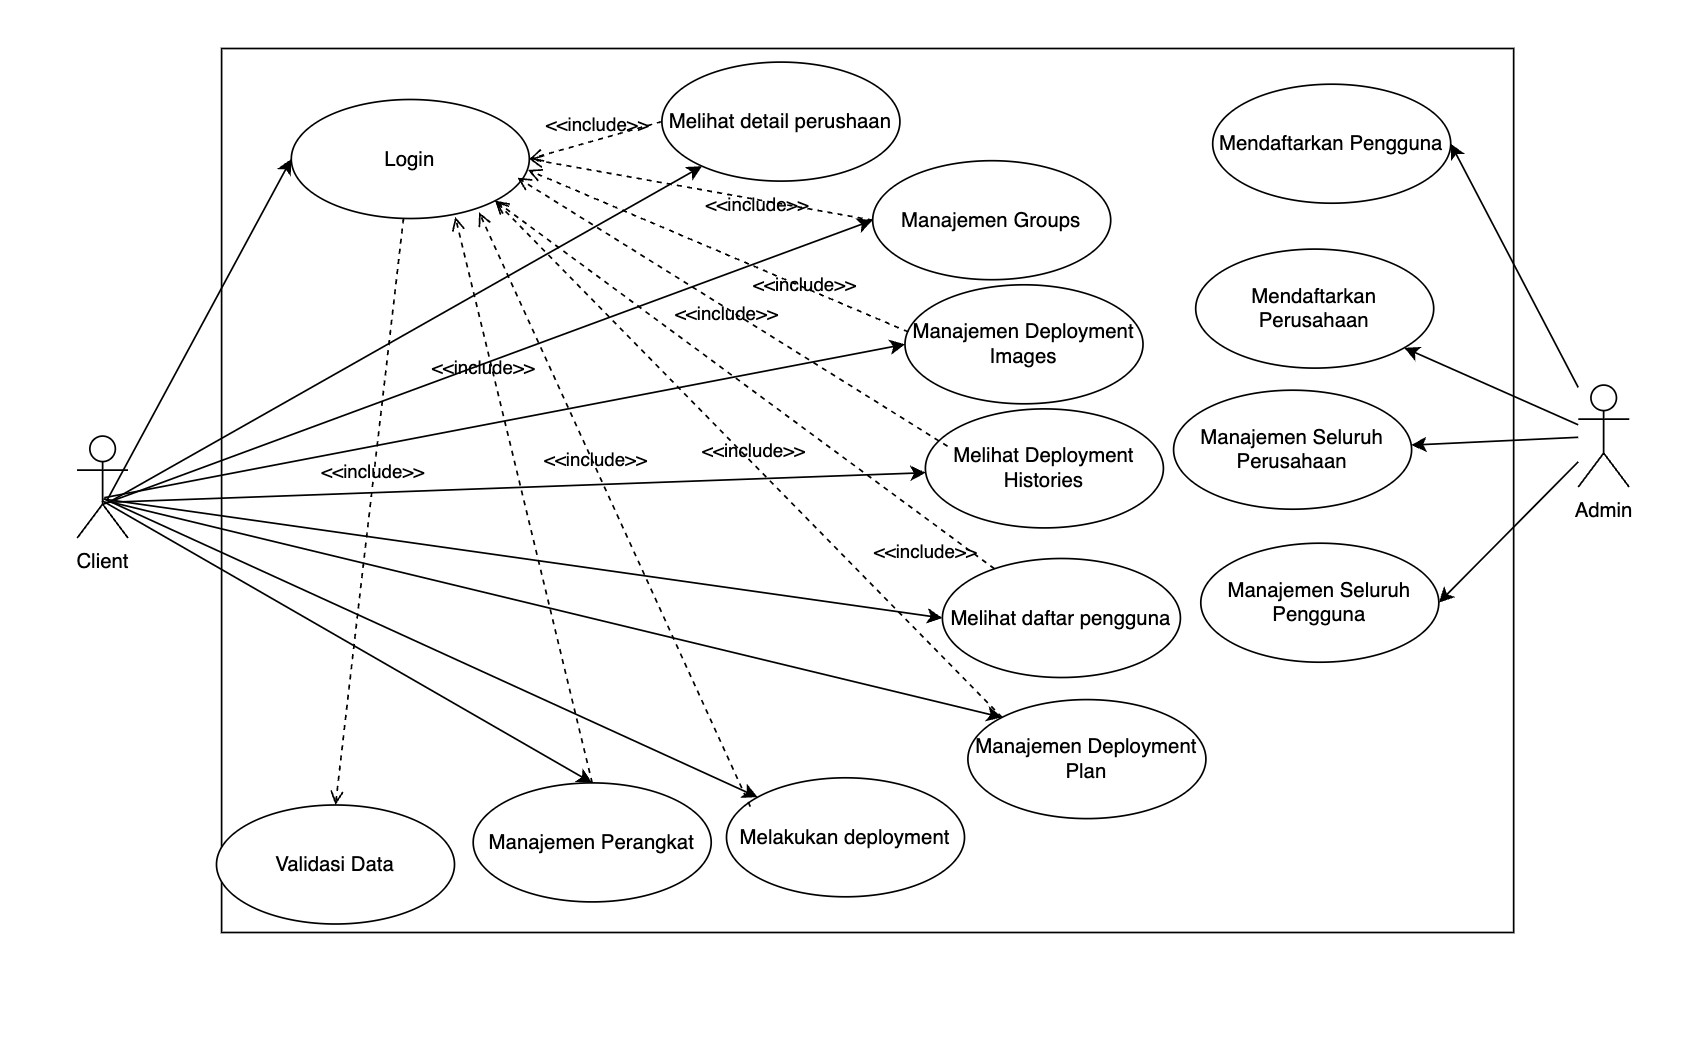
\includegraphics[width=1\textwidth]{resources/chapter-3/usecase-diagram.jpg}
  \caption{Usecase Diagram}
  \label{fig:usecase-diagram}
\end{figure}